\chapter{Control Design and Development}

This chapter presents the arm control design and development that will achieve the objectives highlighted in Section \ref{Design} and illustrated in Figure \ref{fig:bdd}. This journey spans across three stages, each building up from the preceding one, starting from a static control to a sophisticated EMG-influenced control.  

The chapter commences with the \textbf{Static Controller}. This controllers serves as a foundation to ensure the arm's steadiness in a specified position. Utilizing the models from Section \ref{sec:model} and combining it with a PI Controller, the necessary neural activations are generated to hold the arm in the static position. To measure its effectiveness, the controller is assessed across 960 points. From this examination, a select group of \textit{feasible points} are identified. A feasible point signifies that the controller was able to find the corresponding neural activation to sustain a target position uninterrupted for a full second. 

Building upon the static controller, the next phase of \textbf{Path Following Quasi-Static Controller} incorporates the element of motion. The calculated feasible points serve as stepping stones, forming a path designed using the K-Nearest-Neighbours algorithm. This path will be used by the controller to move the arm from point to point, steadily aiming for the end target position.

At the end of the chapter the \textbf{EMG-Influenced FES Controller} is studied. Here, muscle activations are tailored according to the design considerations set in \ref{sec:design considerations}, resulting in a distinct stroke-like movement pattern. A FES device is simulated in this phase. Its objective is to supplement the muscle activation to perform the intended movement. The FES device control dynamically adjusts its output depending on the real-time neural activity data from the triceps. 

By the end of this chapter, readers will have an understanding of the layered process performed to design the simulated EMG-Influenced FES controller of this project. 

\section{Static Controller} \label{NeuralController}

The development of the controller, inspired by the methodologies proposed in the paper \cite{QSC}, aims to determine the optimal muscle excitation to stabilize the wrist's position. The architectural layout of this controller is portrayed on Figure \ref{fig:BDC}.

\begin{figure}[h!]
    \centering
    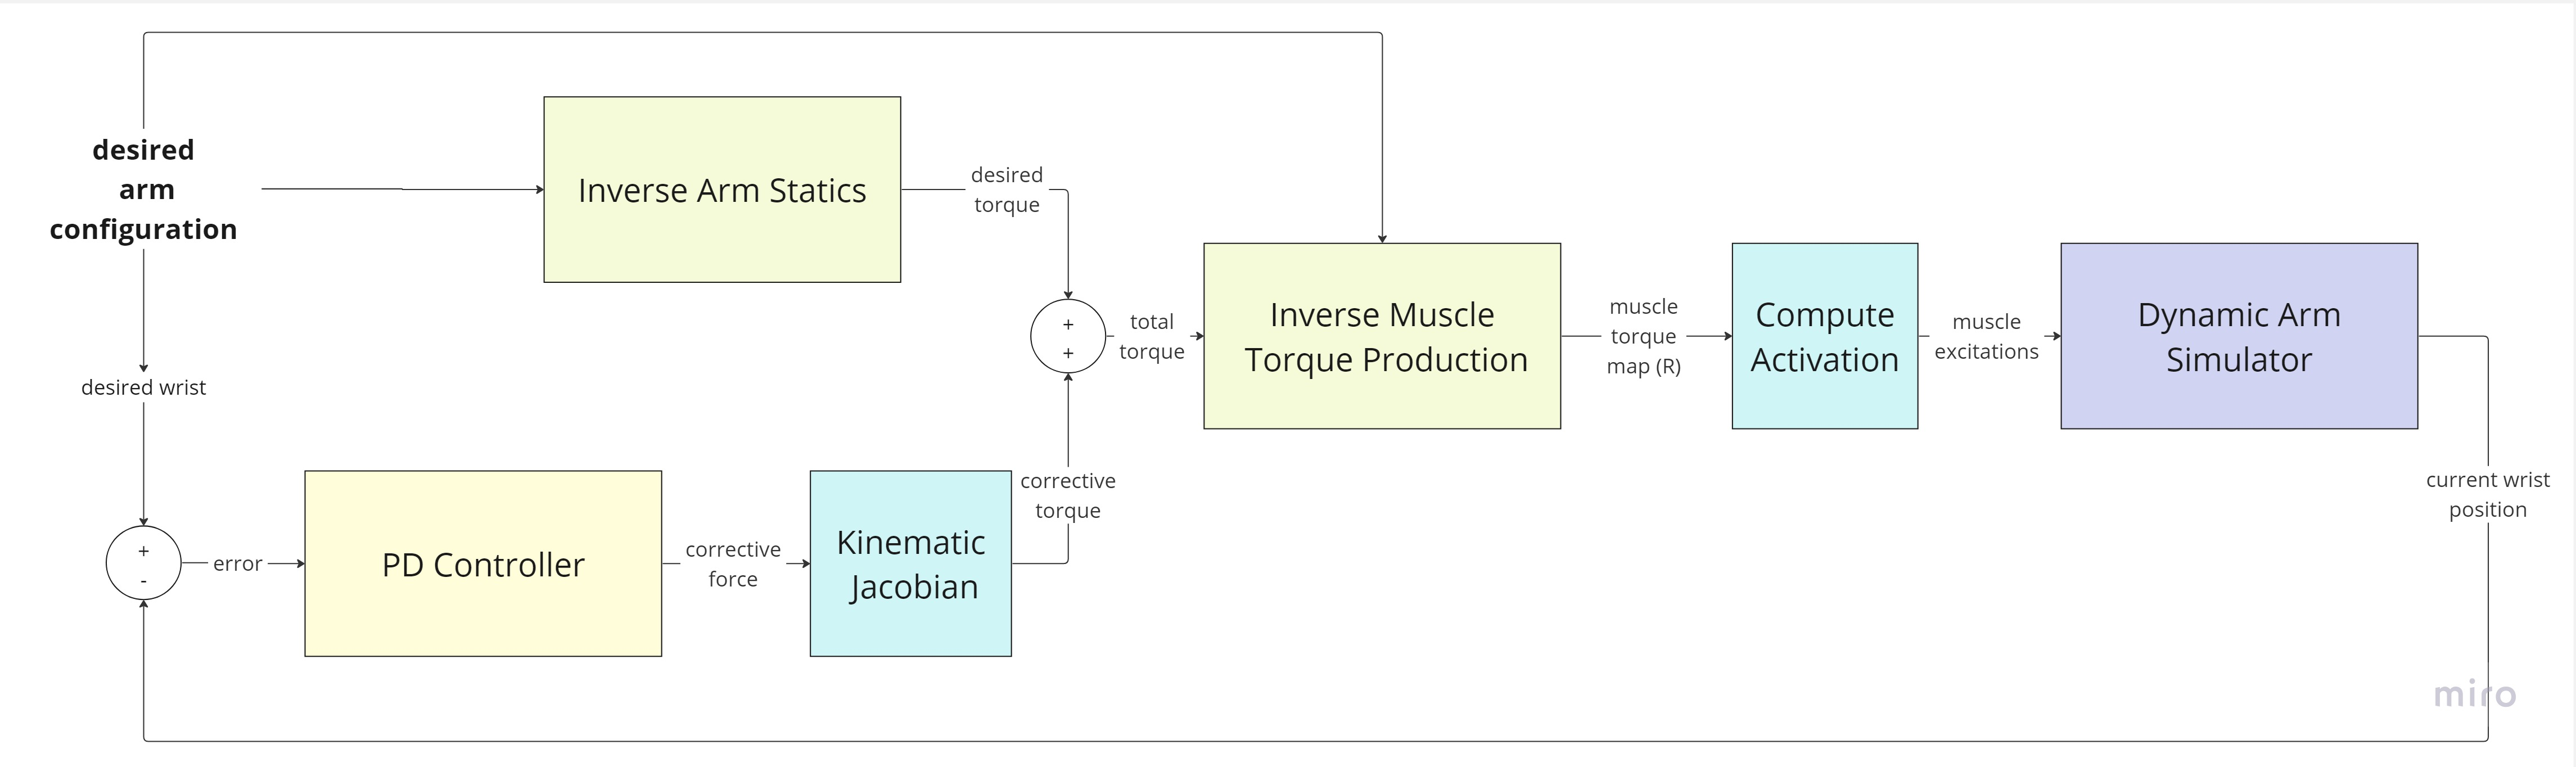
\includegraphics[width=1\textwidth]{Pictures/Controller/controller-diagram.jpg}
    \caption{Controller Block Diagram inspired in \cite{QSC}}
    \label{fig:BDC}
\end{figure}

The input of the controller is the desired arm configuration. Using the Inverse of the Arm Statics model, described in Section \ref{sec:model}, the required torques to maintain the arm in a static position are computed. These torques are subsequently given as an input into the Muscle Torque Production model, elaborated in Section \ref{sec:model}. This model outputs the corresponding muscle excitations which will define the neural excitation input for the Dynamic Arm Simulator. 

The Dynamic Arm Simulator will then determine the arm's dynamics in accordance with the Rosenbrock equation, as explained in Section \ref{sec:dynamics}. Post these dynamic computations, the wrist's actual position is deduced. The error between the desired and the actual wrist position will drive a PI Controller, which will calculate the corrective force needed to match the desired wrist position. The kinematic Jacobian, Section \ref{sec:torque}, will compute the requisite corrective torque. This torque, when combined with the desired torque from the Inverse Arm Statics, provides the total torque which is then input to the Inverse Muscle Torque model, closing the control loop. 


\subsubsection{PI-Tuning}
To assure the PI Controller's performance, an exhaustive hand-tuning was undertaken across 20 different positions, concluding in values of \(K_p = 300\) and \(K_i = 100\). For detailed results see Section \ref{resultsstaticcontrol}.

\subsection{Implementation}

The code below shows the MATLAB implementation of the Static Controller. It is divided into two sections the initial configuration and the simulation loop.

\begin{lstlisting} [style=Matlab-editor-small]
%%%% INITIALIZATION
%Initialize Model
[model, nstates, ndof, nmus, iLce] = initialize_model();

% Initial state
x = x_init; 

% Set Simulation Parameters
tend = 2;
tstep = .003;
nsteps = round((tend-time)/tstep+1;

% Initialize parameters
u=zeros(nmus,1);
handF=[0;0;0];
alpha0 = zeros(8,1);
Moments = zeros(5,1);
exF=[0;0];

% Initialize derivatives and muscle excitations
xdot = zeros(nstates,1);
step_u = zeros(nmus,1);
        
complete = 0;
i = 0;
\end{lstlisting}
\newpage
\begin{lstlisting} [style=Matlab-editor-small]
%%%% SIMULATION
[~, ~, ~, ~, ~, ~, qTH] = das3('Dynamics',x, zeros(size(x)), zeros(138,1));
pose=[qTH;x(10:11)];
while i < nsteps
    i = i+1;   

    % Predict static torque
    staticTorque = predict_static_torque(pose)';
    % Predict activation torque
    M = predict_activation_torque(pose);
    
    % Compute desired torque
    tau_des = tau_feedback + staticTorque';

    % PI Feedback
    Kp = 300;
    Ki = 100;
    
    HandCurrent = wrist_position(x);
    posErr = HandGoal-HandCurrent;
    sumErr=sumErr+posErr*tstep;
    Fk=Kp*posErr;
    Fi=Ki*sumErr;
    Fdes=Fk+Fi;
    
    % Compute torque from Kinematic Jacobian
    [~, ~, ~, ~, ~, ~, qTH] = das3('Dynamics',x, zeros(size(x)), zeros(138,1));
    pose=[qTH;x(10:11)];
    J=computeJacobianDAS_5angles(pose);
    J=J(:,1:4);
    tau_feedback=J'*Fdes;
    
    % Compute Activation
    alpha0 = computeActivation(M,tau_des,alpha0);
    for j=1:9
        mus = muscledict(j);
        u(mus) = alpha0(j);
    end
    
    % Advance simulation by a step
    [x, xdot, step_u] = das3step(x, u, tstep, xdot, step_u, Moments, exF, handF);
end                
\end{lstlisting}

\subsection{Predicting Static Torque and Muscle-Torque Relationship}

To predict the static torque values for an arm configuration ($q (5x1)$), the hyperparameters found for the Gaussian Process Arm Statics model described on Section \ref{sec:model} are used. The resultant torque represent the torque needed to hold the arm static in that configuration.

The muscle-torque relationships \texttt{M} is predicted using the Muscle Torque Production model hyperparameters calculated following the steps explain in Section \ref{sec:model} (see Formula \ref{eq:MAP}). The code gives out a matrix where each column represents the torque for the desired shoulder elevation plane, shoulder elevation, shoulder rotation and elbow flexion produced by each muscle group.

\subsubsection{Implementation}
To calculate the static torque i = 9 in the code below, resulting in a static torque of size 4x1.  When calculating the muscle torque production the code will loop through the 8 muscles (i = [1:8]) giving an output matrix of 4x8.
\newpage
\begin{lstlisting} [style=Matlab-editor-small]
load('modeldata.mat');
q = desired_position;

covGP = {@covSEard};
static_torque = zeros(4,1);
M = zeros(4x8);

muscledata = modeldata.muscle(i);
% for j = 1:4 x= [elevationplane, shoulderelevation, shoulderrotaion, elbowflexion]
covSIMPLEj = {@covj};
covfuncj = {'covSum',{covGP,covSIMPLEj}};
static_torque(j) = gp(muscledata.x.semiparametric.gpHyperparameters, @infExact, @meanj, covfuncj, @likGauss, muscledata.x.semiparametric.trainingInputs, muscledata.x.semiparametric.trainingOutputs, q);
(...)
\end{lstlisting}


\subsection{Predicting Muscle Excitations}\label{computemuscleexcitation}

In muscle-driven systems, accurately determining muscle activation patterns is crucial for understanding force generation. 

The objective is to compute the muscle activation $\alpha_0$ for given muscle-torque relationships $M$, desired torques $\tau_{desired}$, and initial guesses for activations is given. This is represented by the following equation:
\begin{equation}
    \tau_{desired} = M * \alpha_0
\end{equation}

In other words how much activation the different muscle groups need to generate the desired torque. 

The optimized muscle activation solution is calculated employing the quasi-newton method supported by the Armijo rule and a penalty-based approach. This method is inspired by \cite{QSC}.

\begin{itemize}
    \item The \textbf{quasi-newton method} is the iterative method used to find this function´s minimum. As computing the Hessian tends to be computationally expensive, the quasi-newton method builds an approximation of it iteratively. In other words, it uses and approximation of the information of the function's curvature (Hessian) to find the shortest way to the minimum. 
    \item The \textbf{Armijo rule } is a method to decided how big of a step to take when trying to find the lower point of a curve or surface.  The step is halved every time a step is not taken into a direction where the value of the function is reduced as expected. The Armijo rule is used to determine the step size of the quasi-Newton method. 
    \item The \textbf{penalty function} makes sure that the muscle activations are withing the range of [0,1], including constraints to the quasi-Newton method. 
\end{itemize}

By employing, the quasi-Newton methods, the function efficiently converges to the optimal solution. The figure below shows how it converges in two random moments of the steps of the simulation. The plots show a sharp decline and then flattens, indicating that the optimization is converging.


\begin{figure}[h]
    \centering
    \begin{subfigure}[b]{0.45\textwidth}
        \centering
        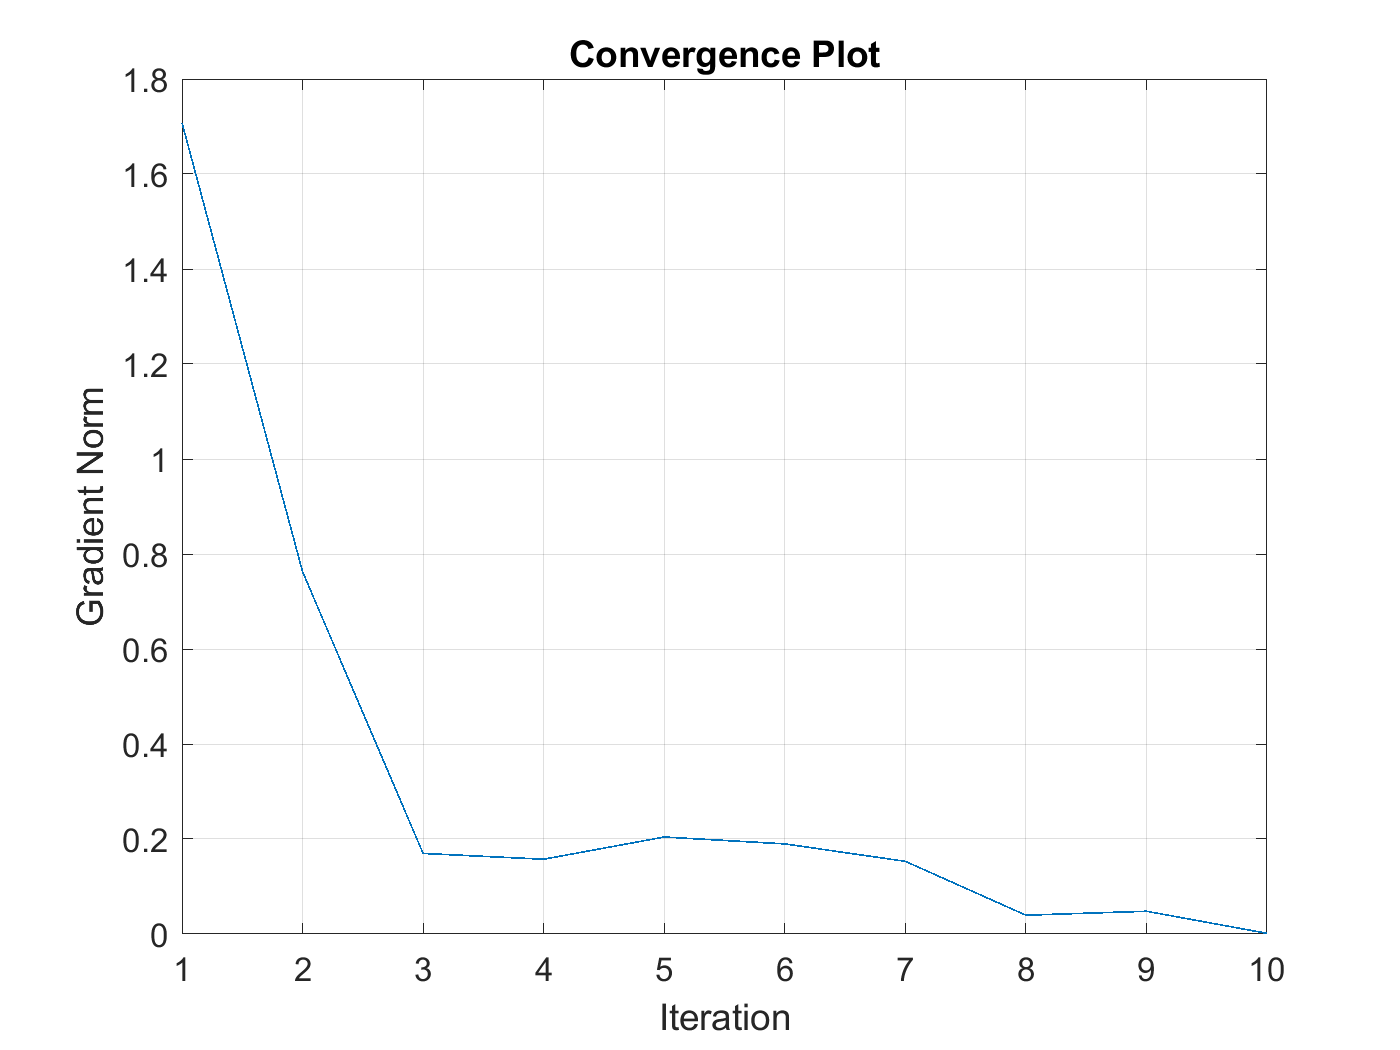
\includegraphics[width=0.8\linewidth]{Pictures/Model/convergence.png}
    \end{subfigure}%
    \hfill
    \begin{subfigure}[b]{0.45\textwidth}
        \centering
        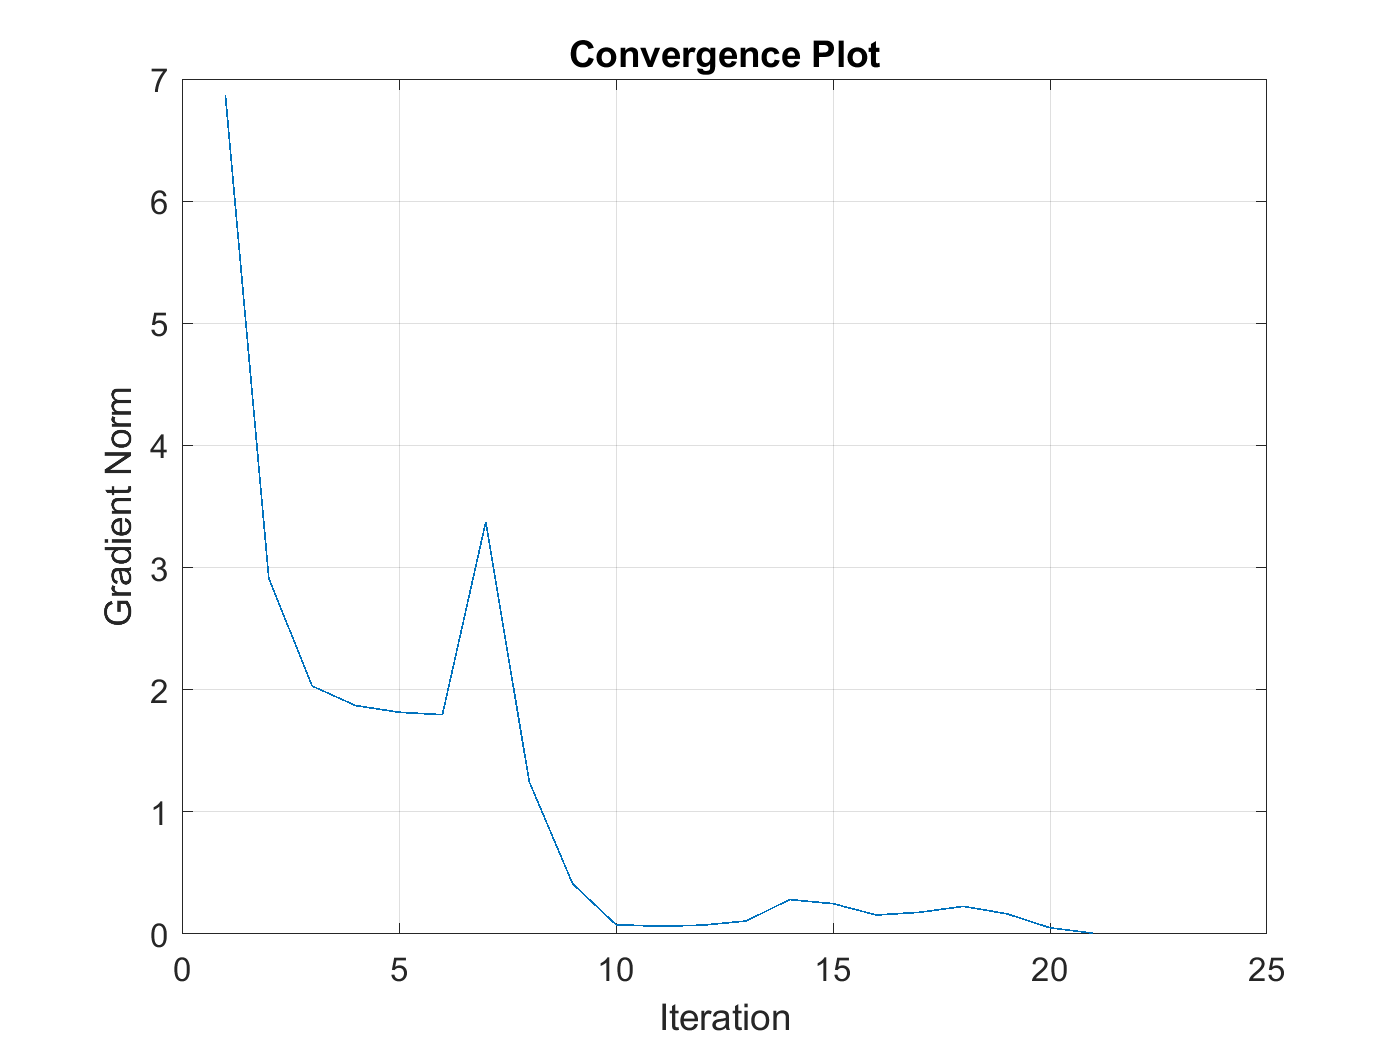
\includegraphics[width=0.8\linewidth]{Pictures/Model/convergence2.png}
    \end{subfigure}
    \caption{Convergence Plot: Gradient Norm vs Iteration}
\end{figure}
\subsection{Feasible Points}
With this tuned controller, a grid, encompassing 960 points, was generated using the \textbf{create\_grid} function (refer to Section \ref{sec:tp}). Each point's arm configuration was calculated using the PI force controller, as detailed in Section \ref{sec:PI}. The feasibility of a point was determined by the ability of the controller to sustain for 1 second its position with an error margin of 0.1. For clarification purposes, the start and the goal position of the controller are set to be the same. 
For seamless and accurate operations, a time step (\(t_{step}\)) of 0.001 is employed. To improve the controller's stability an auxiliary force is exerted on the arm in the first 100 steps. This eliminates potential oscillations and assures a better control performance.

The figures (gif if opened in Adobe Acrobat) below present the generated grid. Points in red signify positions where the controller failed to find the neural excitation needed to sustain for 1 second. In contrast, green points indicate successful stabilization by the controller. These feasible points will be used in the following section (Section \ref{sec:path}) to generate paths for the arm to follow. 


\begin{figure}[ht]
    \centering
    \animategraphics[autoplay,loop,width=0.8\textwidth]{12}{Pictures/Controller/gif/feasiblepoints-}{0}{149}
    \caption{Feasible points. Open in Adobe Acrobat to see gif movement.}
    \label{gif:Feasiblepoints}
\end{figure}

\newpage
\section{Path Following Quasi-Static Controller Development } \label{sec:path}

The goal is to develop a controller that allows the dynamic arm  to navigate or follow a specific trajectory or path. This will simulate the rehabilitation reaching task to be performed. For more information on rehabilitation tasks refer back to Section \ref{rehabilitation_task}. Quasi-static control allows to design a safe, precise and movement-controlled therapy, as it focuses on slow, steady and controlled operations. It facilitates the decomposition of the entire reaching path trajectory into smaller static positions. Dividing the task into smaller steps offers some benefits under the rehabilitation lens:
\begin{itemize}
    \item \textbf{Gradual Progression}. Rehabilitation often demands gradual approach towards exercises, specially for recovering patients. progress.
    \item \textbf{Progress Tracking} Breaking the movement into smaller steps helps not only patients to progress at a comfortable and safe pace but allows to keep track of the progress.
    \item \textbf{Minimized Fatigue} Continuous motions can take a toll in patients with limited strength and endurance. Smaller tasks reduce muscle and join strain preventing fatigue. Using a quasi-static controller can help modify the parameters to adjust to the patient's abilities. 
\end{itemize}

\begin{figure}[h!]
    \centering
    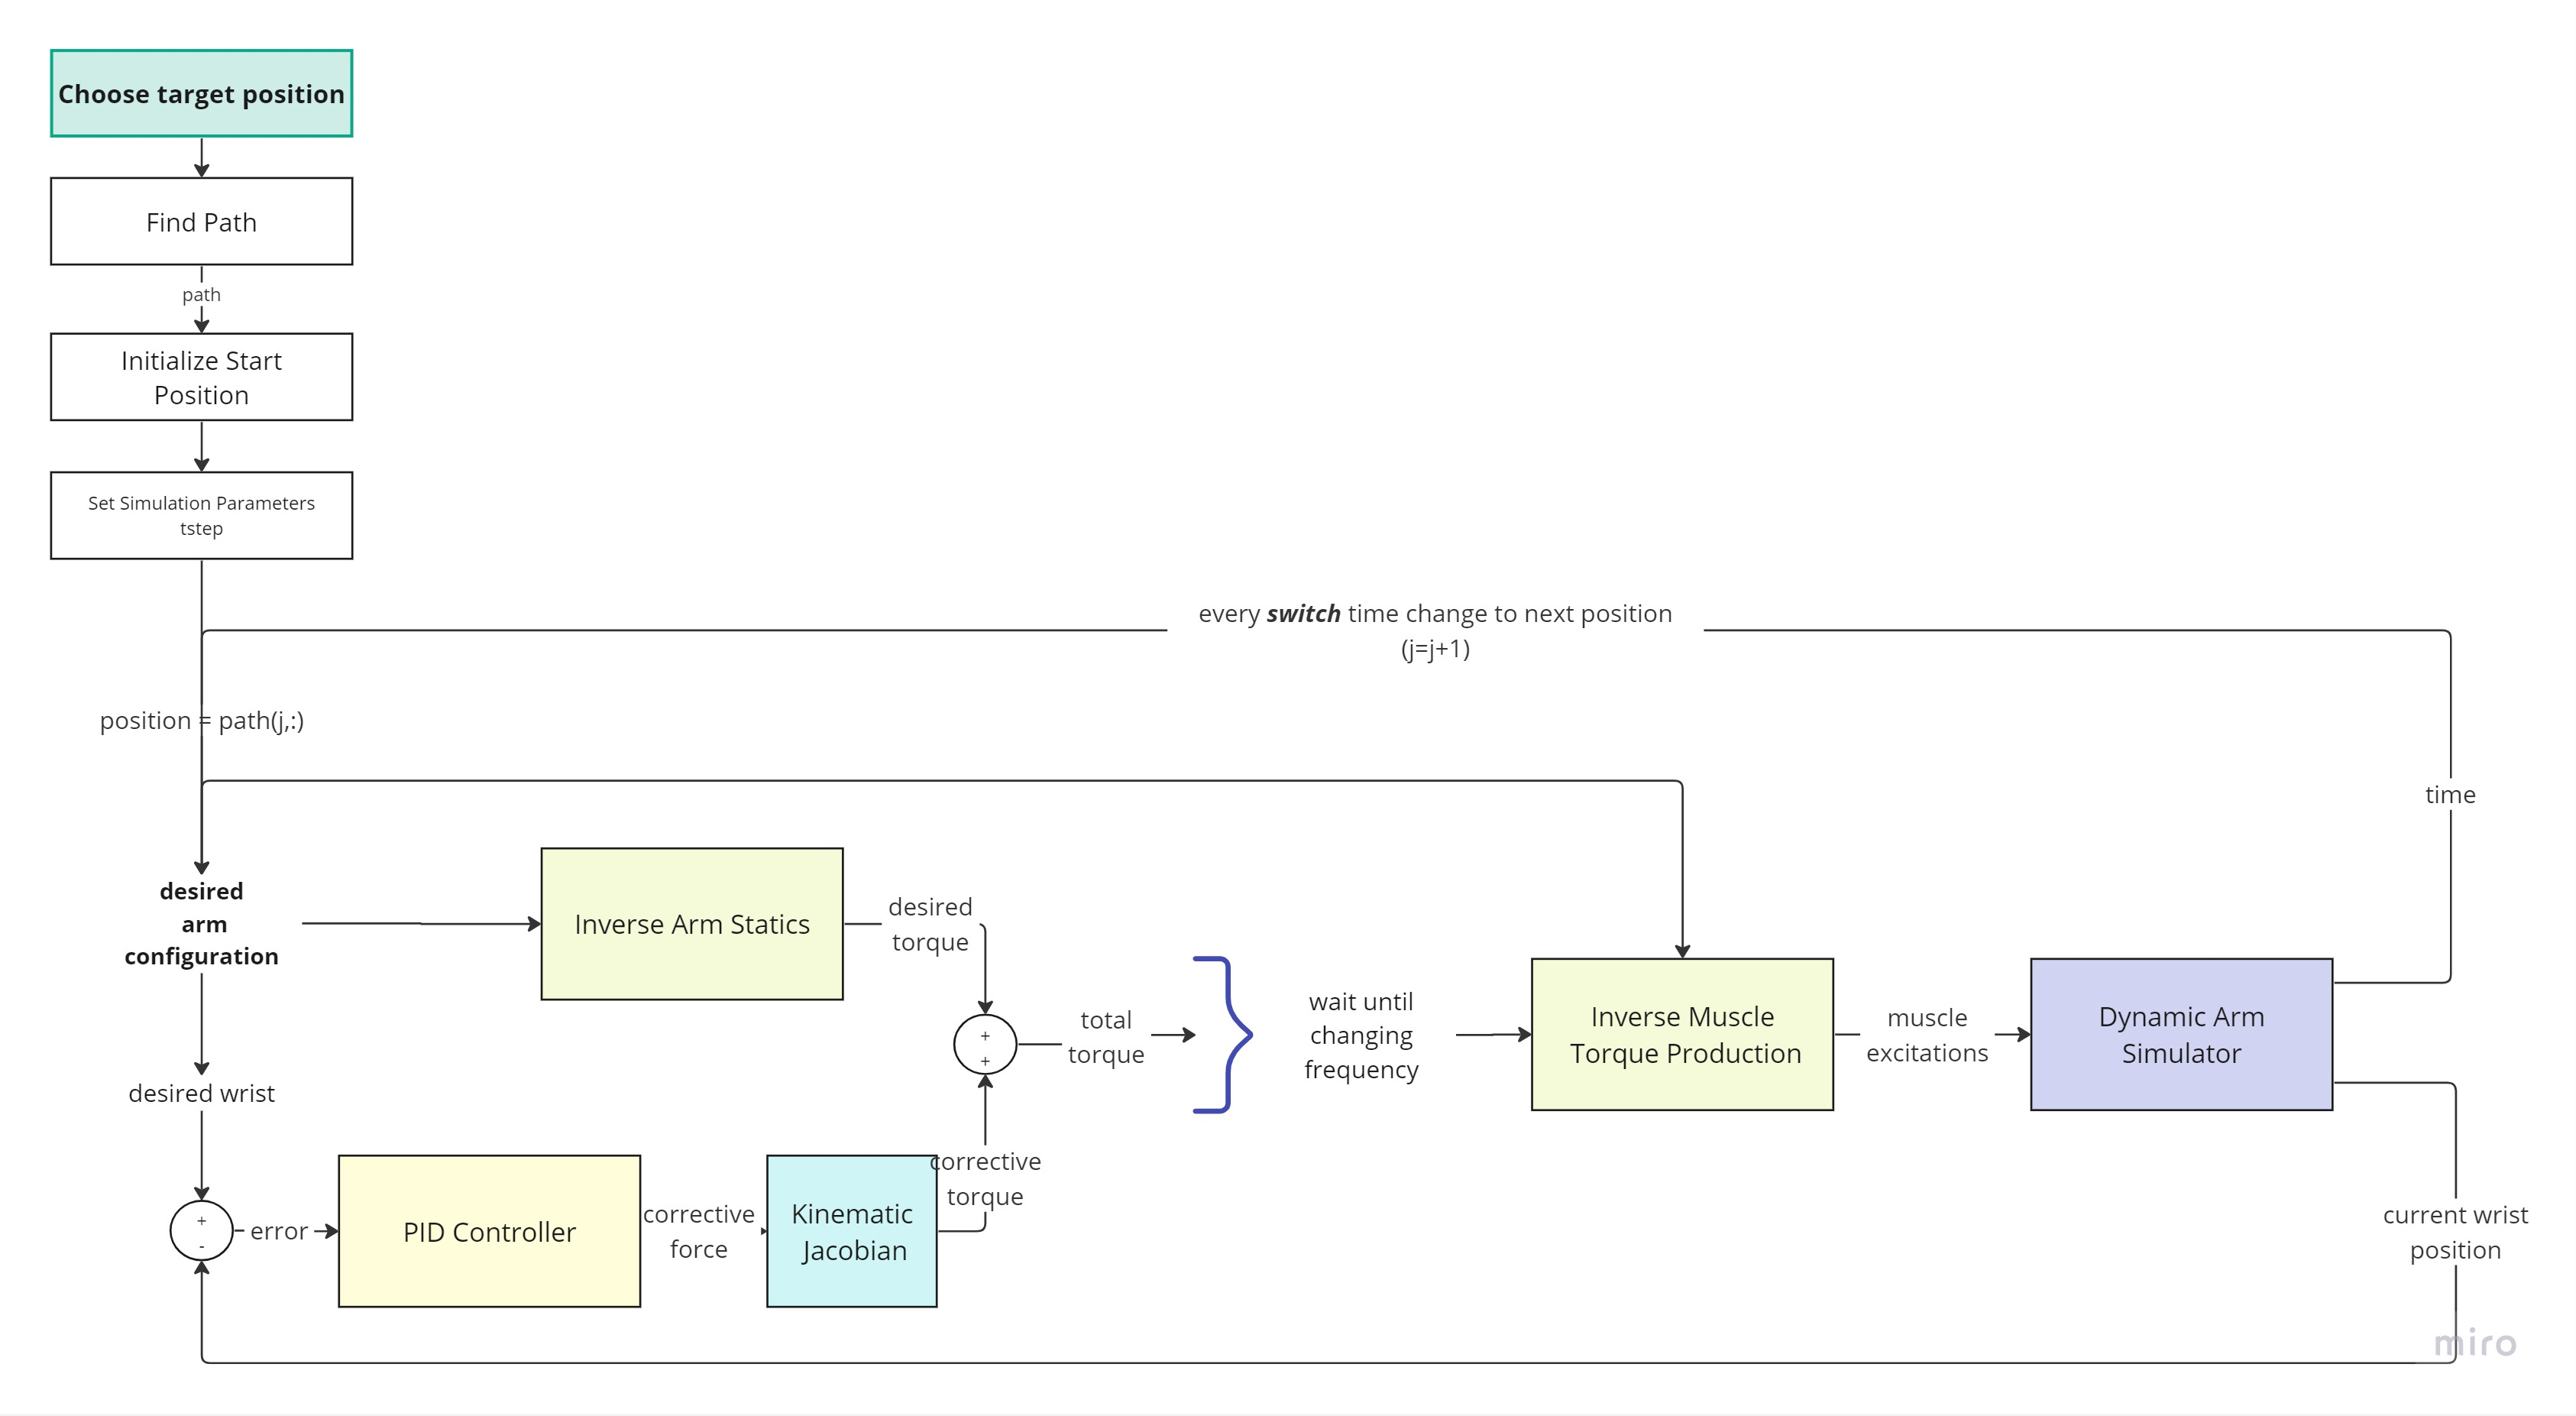
\includegraphics[width=1\textwidth]{Pictures/Controller/Quasi-Static Path Controller.jpg}
    \caption{Flow Diagram Quasi-Static Path Controller }
    \label{fig:PathController}
\end{figure}
\newpage
For a clearer understanding of the quasi-static control designed, refer to the flow diagram included in this chapter (Figure \ref{fig:PathController}). Here’s a descriptive step-by-step breakdown of the process of path controller:

\begin{enumerate}
    \item \textbf{Selection of Target Position}: From a set of feasible points, a target position is chosen. This serves as the end-point or goal for the system.
    
    \item \textbf{Path Discovery via the 'find path' Function} (see Section \ref{findpath}, for a more detailed explanation of the function): The selected target position is input into the 'find path' function. This function works by first identifying the nearest neighbors from the feasible points workspace. Among the first 200 nearest neighbors of the starting point, it selects one that:
    \begin{itemize}
        \item Is at a distance \(d = 4\) units away from the starting point. This distance recommendation comes from the paper \cite{QSC}.
        \item Lies in the direction of the end-point or target position.
    \end{itemize}
    Through this method, a path consisting of multiple positions is generated.
    
    \item \textbf{Setting Initial Simulation Parameters}: At the beginning of the simulation, the initial position from the path is defined. Moreover the simulation parameter are set: \(t_{step} = 0.003\), and a $frequency$ of 30Hz. The variable $frequency$ refers to the rate at which the FES (Functional Electrical Stimulation) device can change its input. This is a criteria detailed on the design Section \ref{Design} limited by the FES devices.
    
    \item \textbf{Control Loop}: The control loop operates as previously outlined in the Section \ref{NeuralController} , with a few distinct modifications:
    \begin{itemize}
        \item \textbf{Neural Excitation}: This only takes place at set intervals based on the defined $frequency$.
        \item \textbf{Position Switching}: At every $time_{switch}$ the position in the control system is updated to the subsequent one in the predefined path array.
        
        If the hand has not reached the vicinity of the targeted position within the set time frame of $time_{switch}$, the system will attempt to reach the position a maximum of two more times before potentially moving to the next point or terminating.
    \end{itemize}
\end{enumerate}

In conclusion, the proposed controller is designed to guide a dynamic arm through specified trajectories, mimicking the rehabilitation reaching tasks outlined in Section \ref{rehabilitation_task}. Quasi-static control is used to emphasize safety, precision and control, three key components for a successful rehabilitation. Key components of the control system presented include a \textbf{\textit{find\_path} }function that uses KNN to find the best positions that will define the path to the desired target. Moreover the control loop, adapted from the one on Section \ref{NeuralController}, operated with timed neural excitation (controlled by the variable $frequency$) and position switching to guide the arm accurately along the predefined path (controlled by variable $time_{switch}$).




\subsection{Find Path Function} \label{findpath}

The \texttt{FindPath} function calculates a path between two positions within a predefined set of feasible wrist points. The function takes three input parameters: $d$,  $startPos$ and $endPos$. 

The code will load a file that contains all the feasible wrists positions to calculate a path from. Section \ref{NeuralController} explains how the feasible positions are determined. 

Once all the initial parameters are set, the function begins to construct the path. K-Nearest Neighbours is the supervised machine learning algorithm used to calculate the most optimal path. The Matlab function \textbf{knnsearch} is used to seek the predefined number of nearest neighbours to the current position within the feasible positions. Then, another \textbf{knnsearch} is performed to identify which one of the closest neighbours is closer to the end position. The selected point should be within a distance $d$ from the current position but closet to the end position.

This process is repeated until the path reaches the desired end position. As a result, find path outputs an array called path will all the positions.


\begin{figure}[h!]
    \centering
    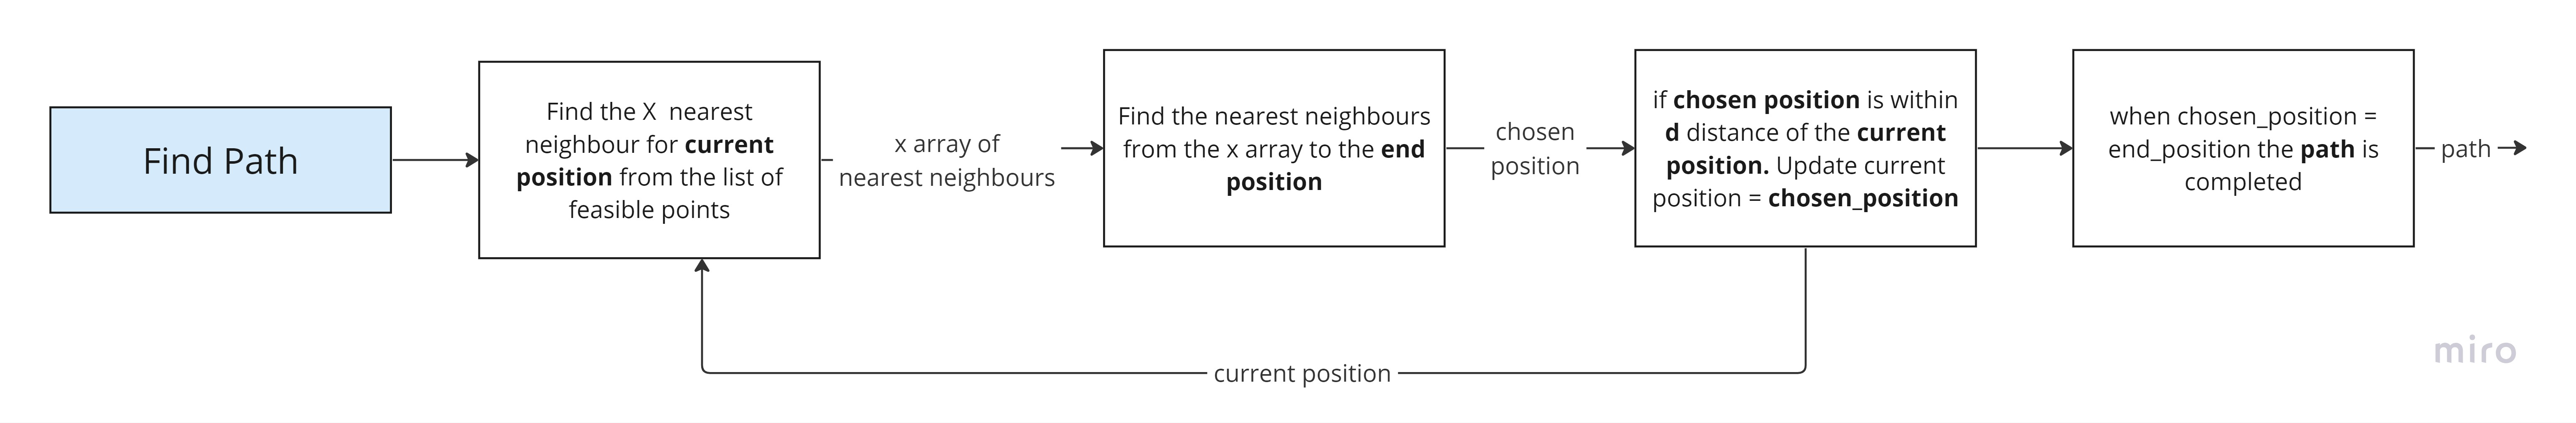
\includegraphics[width=1\textwidth]{Pictures/Controller/findpath.jpg}
    \caption{Flow Diagram Find Path Function }
    \label{fig:FindPath}
\end{figure}

\subsection{Implementation}
The Matlab code implements the Path Following Quasi-Static Controller . 

\begin{lstlisting} [style=Matlab-editor-small]
%%% INITIALIZATION same as Static Controller 
(...)
switchTime = 1.3;
startPos = x; 
endPos = target;
d = 4; 
last = 0;
pathIdx = 2;
(...)

path = FindPath(d, startPos, endPos);

%%% SIMULATION 

while last = 0
    (...) % Same as Static Controller
    GoalPos = path(pathIdx);
    if mod(i,floor(switchTime/tstep))==0
        HandCurrent = wrist_position(x);
        distance = norm(HandGoal-HandCurrent);
        if distance < 0.05 || trial >0 
        if pathIdx < length(path)
            pathIdx=pathIdx+1;
        else 
            last =1; %last point in path
        end
        GoalPos = path(pathIdx);
        [~, ~, ~, ~, ~, ~, qTH] = das3('Dynamics ',GoalPos, zeros (size(x)), zeros
        (138 ,1));
        pose =[ qTH; GoalPos(10:11)]
        
        % Predict static torque (...)
        % Predict activation torque (...)
    end
    % PI Feedback

    if mod(i,frequency)==0
        %Compute Activation (...)
    end

    %Advanced simulation by a step (...)
    
\end{lstlisting}


\newpage
\section{EMG-Influenced FES Controller Development}

Building on top of the controllers previously designed and discussed in this section, the investigation is extended into the intricate challenges faced by stroke patients. An after-math of stroke is the muscular imbalances, most specifically muscle spasticity, which refers to muscle stiffness that influences movement and speed. As a result, they present difficulty extending the arm. The biceps tend to be over-activated and the triceps and anterior deltoid under-activated \cite{IOL}. To counteract these muscular imbalances, this controller has being design to simulate an effective and targeted electric stimulation. 

Two key additions are included in the following controller design:

\begin{enumerate}
    \item a component that emulates the over activity of the biceps post-stroke 
    \item the addition of FES to activate the triceps
\end{enumerate}

A complete flow diagram is portrayed on Figure \ref{fig:FESController}.

\subsection{Emulating Biceps Over-Activity}

The code segment initiates by calculating muscle activation levels using the \textbf{\textit{computeActivations}} function, which factors in muscle force models and desired torques  (refer to Section \ref{NeuralController}). Then, it proceeds to iterate through the set of  muscles. When the loop reaches the biceps, the activation level of the biceps is modulated by a factor termed \textbf{\textit{stroke}}, representing the over-activity induced due to the stroke condition. This modulation is subsequently bounded: if the resultant activation surpasses a threshold of 1, it is capped at this upper limit. In scenarios where the activation is null and the stroke factor exceeds 1, a minimal activation level of 0.3 is set to ensure a base activation. For each iteration, the modified activation values are assigned to the corresponding muscle index in the control input vector u. It is important to highlight that the values are only updated with respect to the FES frequency (concept explained in Section \ref{sec:path}).

\subsection{FES Stimulator for the Triceps}

Considering the biomechanical implications, this project focuses on applying the Functional Electrical Stimulation the triceps. The control examines the triceps activation levels. This information comes from the Dynamic Arm Simulator and in a real case scenario it will come from EMG sensors situated in the triceps of the human. 

If no activation is detected, a default minimal value is assigned. However, in cases with existing activation, a sigmoid-based control system is adopted. 
\begin{equation}\label{sigmoid}
    \sigma(z) = \frac{1}{1 + e^{-z}}
\end{equation}

This methods adapts the gain in a smooth manner between predefined boundaries, allowing for a nuanced control response that remains sensitive to the velocity-driven nature of spasticity.

For correct simulation it is ensured that the triceps activation remains bounded between [0.2, 1]. 


\newpage
\begin{landscape} % Start landscape page
  \begin{figure}[h!]
    \centering
    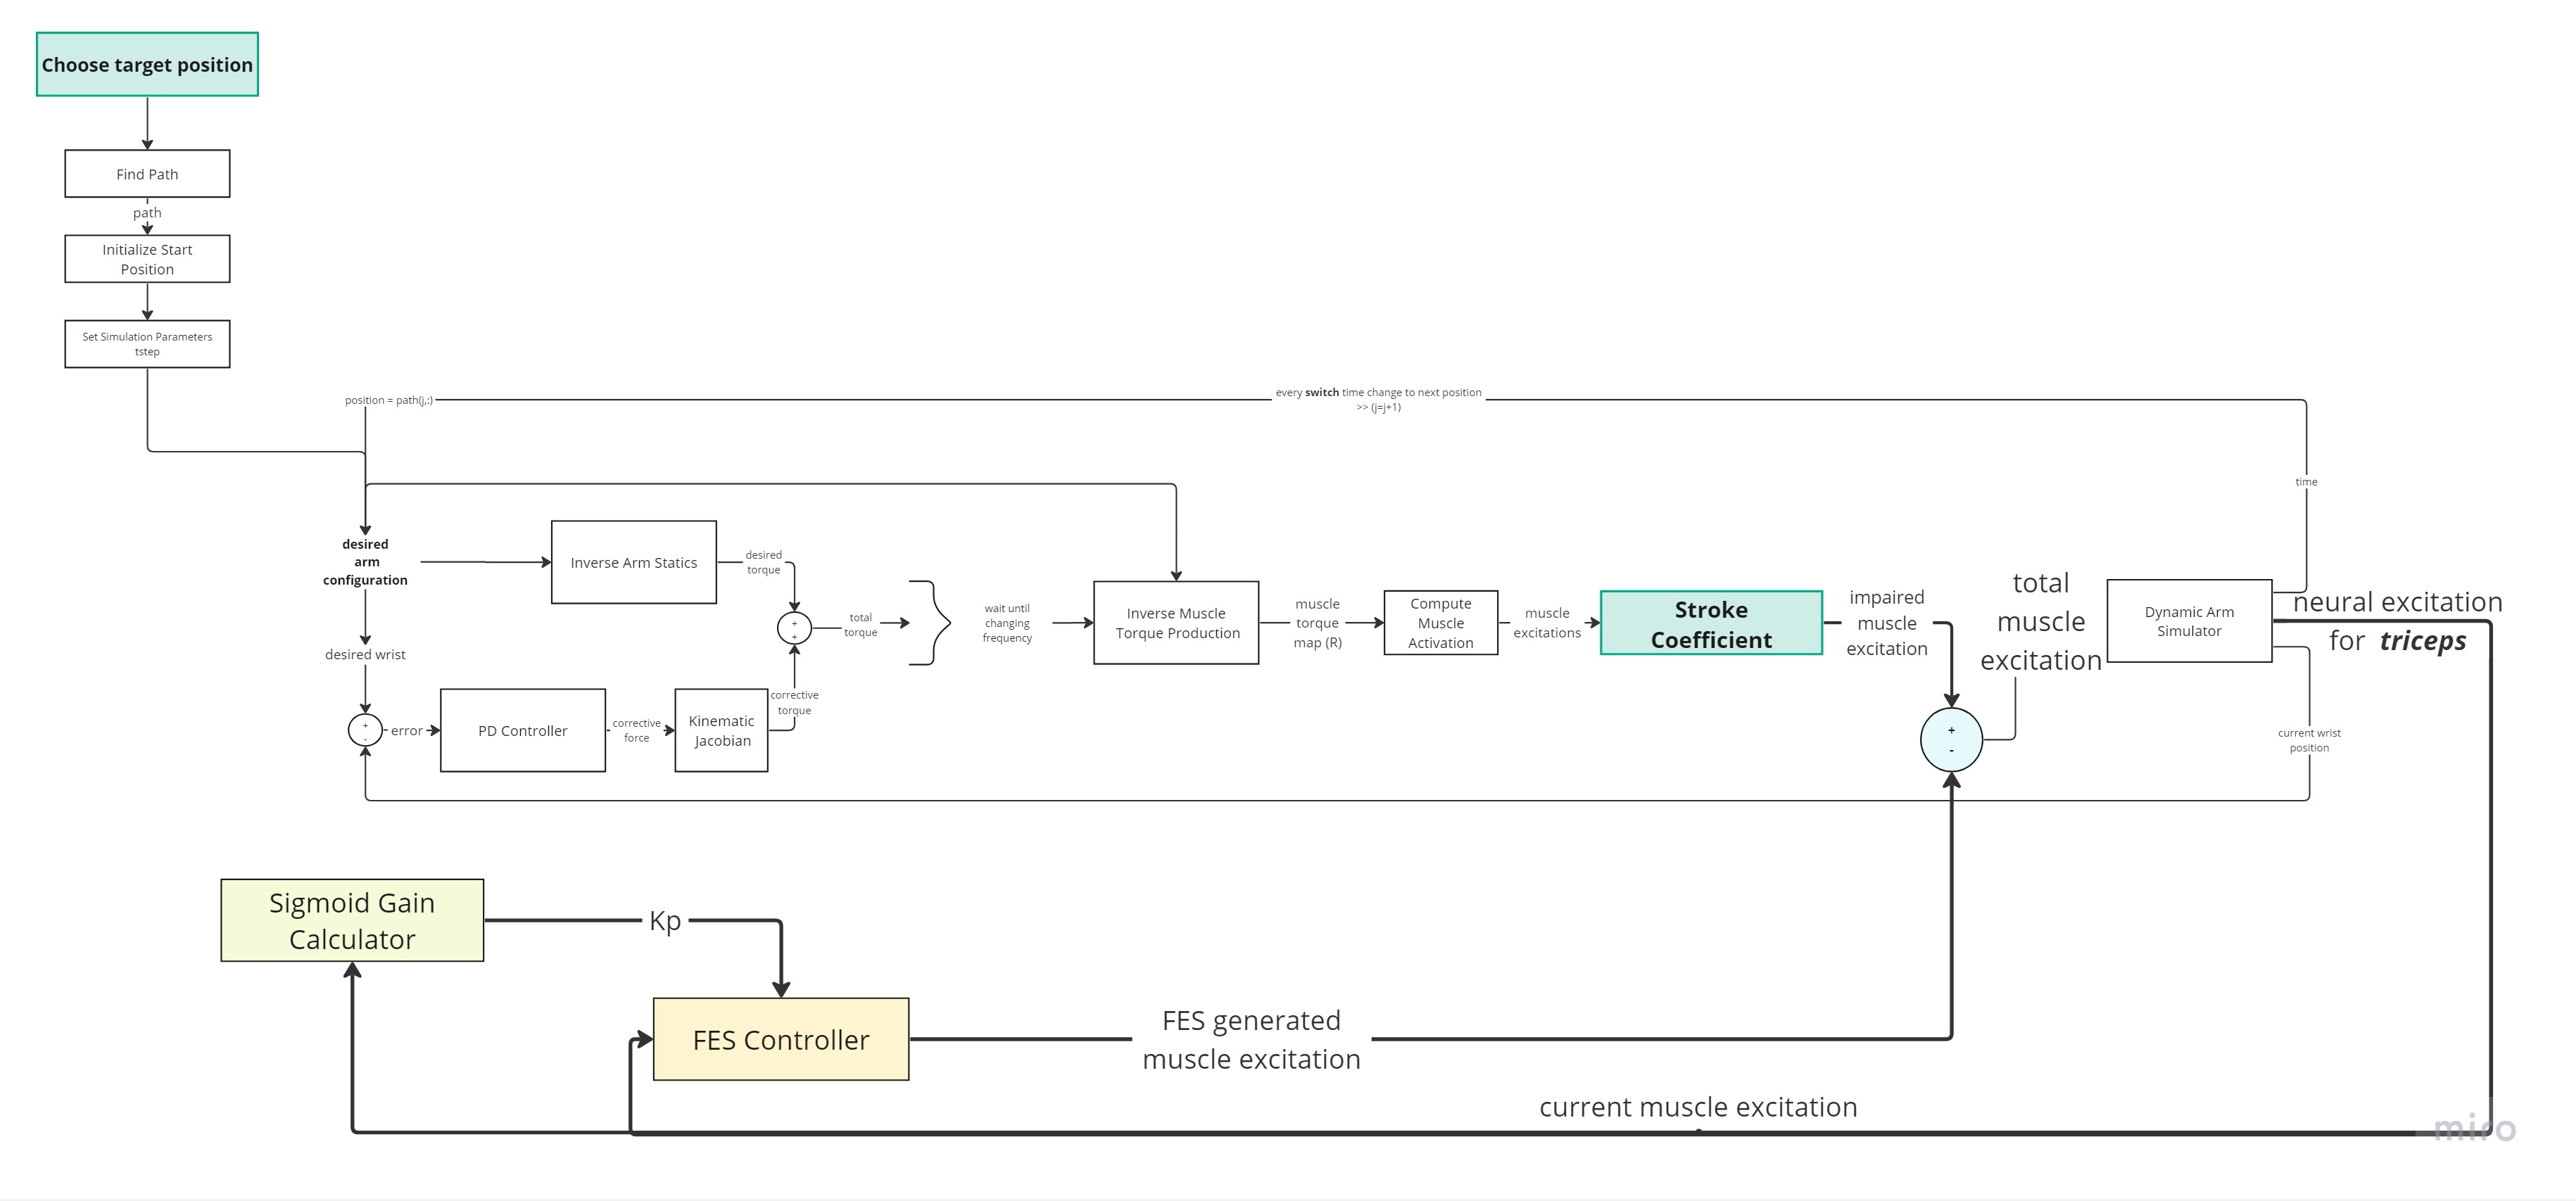
\includegraphics[width=1.7\textwidth]{Pictures/Controller/FESController.jpg} % Replace "filename.jpg" with the name of your image file
    \caption{Flow Diagram for EMG-influenced FES Controller} % Optional caption
    \label{fig:FESController} % Optional label for referencing
  \end{figure}
\end{landscape} % End landscape page

\subsection{PD Controller Tuning: Simulated Annealing}


Building on the insights from the study by \cite{PDP}, where they refine the performance of a proportional derivative controller for a two-segment planar arm model, simulated annealing is used to tune the gains of the FES controller. 

The core idea is to identify the best controller gains for the sigmoid function (Equation \ref{sigmoid}) by minimizing the positional error over time. This error was quantified by the formula:

\begin{equation}
f_{error} = \sqrt{\frac{1}{2TN_m}\sum_{i=1}^{N_m}\sum_{j=1}^{3}\int_{0}^{T}(\varphi_{ij}(t)-\varphi_{ij}^{target})^2 dt}
\end{equation}

Here, $\varphi_{ij}(t)$ represents the wrist's current position in either x, y, or z coordinates, while $\varphi_{ij}^{target}$ indicates the desired wrist position. The term $T$ specifies the movement's time span, and $N_m$ denotes the 10 arbitrary movements carried out during the simulation.

To calculate the optimal values, simulated annealing algorithm \cite{SimulatedAnnealing} was utilized. Simulated annealing is a probabilistic technique for approximating the global optimum of a given function. It seeks to find the best solution. 

It begins with a initial solution which is set to an initial high temperature. This temperature will control the likelihood of accepting worse solutions as the algorithm progresses. At each iteration a neighbouring solution is chosen randomly. If the neighbouring solution is better than the current one it is accepted as the new current solution. If it is worsen it may accept it depending on the temperature and the difference in quality of accepting the solution or not. After each iteration the temperature is cooled down following the cooling schedule. 


The Matlab function \textbf{simulannealbn} is used with the default annealing function \textit{annealingfast}. This function represents how the new points are generated for the next iteration. In this case it has a step with the length temperature (higher temperature higher step) and with a direction uniformly at random. The temperature function used is \textit{temperatureexp}, an exponential decay where the temperature is multiplied by a factor between 0 and 1. The algorithm stops when the temperature reaches a predetermined minimum value, after a fixed number of iterations. 

Simulated annealing avoids getting trapped in local minima, as early on when the temperature is higher the algorithm is more willing to accept worse solutions. In other words, as the temperature cools down the algorithm becomes more selective. 

For this project purposes, maximum of 100 iterations is stipulated, a fixed a function tolerance at 1e-3, and an initial estimate of [10 1.3] for the sigmoid function's two gains  is provided.. The bounds for the controller gains were set between [1.2 3] and [3 15].

The simulated annealing successfully calculated the proportional value to be equal to [2.99 14.478].

\begin{figure}[h!]
    \centering
    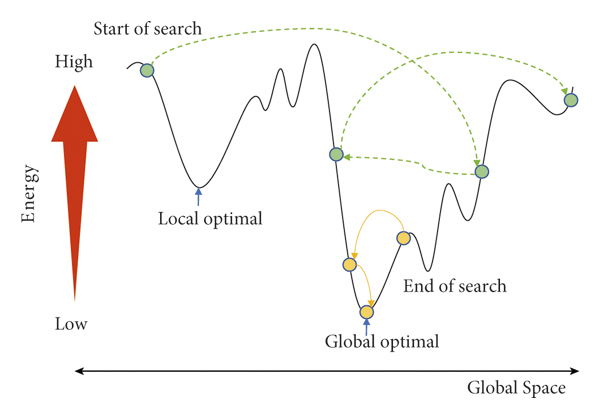
\includegraphics[width=0.6\textwidth]{Pictures/Controller/simulated_annealing.jpg}
    \caption{Simulated Annealing Explanatory Diagram \cite{SANN}}
    \label{fig:simulatedannealing}
\end{figure}
